\scanpage{43}
avec le torseur $P_s$ sous $G_{k(s)}$ et la trivialisation $p(x)\in P_s(\mathbb{C})$.

En termes de $\unsure{w|\omega}$ et $q:\bar S_{\mathbb{C}}\longrightarrow P_{\mathbb{C}}^{\mathrm{an}}$, la donnée de $f$ revient à la donnée de
\[
f:\bar S_{\mathbb{C}}\longrightarrow\unsure{\gamma|\mathscr{Y}}_G
\]
satisfaisant les conditions

a) $f$ holomorphe

b) $f(xg)=w(g)^{-1}f(x)$

c) \deleted{$\unsure{f(\xi_0)|f(\bar\xi_0)}$} $\forall\bar s\in\bar S_{\mathbb{C}}$, \inserted{sur $s\in S$} $f(\bar s):\mathbb{S}\relbarG_{\mathbb{R}}$ est compatible avec le torseur $P_s$ sur $G_{k(s)}$ et sa trivialisation $q(x)\in P_s(\mathbb{C})$.

Enfin, \deleted{pour tout $k$}, on se donne une ``\unsure{restiction|restriction}'' du rev. $\widetilde{\mathbb P}_{\mathbb{C}}\mathbin{\times}^{G(\mathbb{Q})}G(\mathcal A)\deleted{\mathbb{Q}_{\ell}}$ sur $S_{\mathbb{C}}^{\mathrm{an}}$ en un revêtement
% slanted
\margin{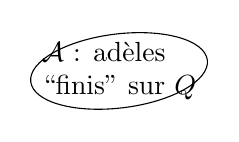
\begin{tikzpicture}[baseline=(current bounding box.center)]
\node[inner sep=0pt,align=left] (note) {$\mathcal A$ : adèles\\``finis'' sur $\mathbb{Q}$};
\draw[rotate around={7:(note.center)}] (note.center) ellipse [x radius=1.13cm,y radius=.47cm];
\end{tikzpicture}}
\deleted{sur $S$ dont de \unsure{gpe|grp} $G_\ell$} de groupe $G(\mathbb{Q}_{\ell})$ sur $S$, En termes \inserted{de $\xi_0$ et} de $\Gamma=\pi_1(S(\mathbb{C}),\unsure{\xi|\mathord{)}}_0)$, on se donne une factorisation de $\Gamma\xrightarrow{w}G(\mathbb{Q})\relbarG(\mathcal A)$ par $\Gamma\longrightarrow\Pi_1\underset{\substack{\Vert\\\Pi_1}}{(S},\xi_0)\longrightarrow G(\mathcal A)$. Quant au revêtement $\widetilde P_{\mathbb{C}}\mathbin{\times}^{G(\mathbb{Q})}(\deleted{\unsure{G|\mathcal A}}\mathcal A/G^{\unsure{0|\circ}})(\mathcal A)$, \deleted{égal à $\widetilde P_{\mathbb{C}}\times$}\inserted{il est} associé à $\widetilde P_{\mathbb{C}}/G^0(\mathbb{Q})\deleted{\text{de}}\unsure{=|\relbar}(P/G^0)_{\mathbb{C}}^{\mathrm{an}}$, \deleted{\unsure{qui|qu'}}et \unsure{à|:} ce titre \unsure{leur|leurs} restriction à $S$ \deleted{\unsure{est|et}} est connue. On veut que ce sont celles données plus haut.....

\deleted{\uline{NB} \unsure{L'application|l'application} $f$ \unsure{est|et}}
% archive sheet number: 42
